\documentclass{beamer}
\usetheme{Warsaw}

\usepackage[T1]{fontenc}%
\usepackage[utf8]{inputenc}%
\usepackage[main=francais,english]{babel}%

\usepackage{graphicx}%
\usepackage{url}%
\usepackage{amsmath}
\usepackage{mathpazo}%
\usepackage{amssymb}

\newcommand{\uconcat}{\ensuremath{+\!\!\!+\,}}

\DeclareMathOperator{\proj}{\mathchar"1119}
\DeclareMathOperator{\sel}{\mathchar"111B}
\DeclareMathOperator{\frag}{frag}
\DeclareMathOperator{\defrag}{defrag}
\DeclareMathOperator{\crypt}{crypt}
\DeclareMathOperator{\decrypt}{decrypt}
\DeclareMathOperator{\group}{group}
\DeclareMathOperator{\id}{id}
\DeclareMathOperator{\dom}{dom}
\DeclareMathOperator{\ens}{E}
\DeclareMathOperator{\R}{R}
\DeclareMathOperator{\Sc}{S}
\DeclareMathOperator{\s}{sch}
\DeclareMathOperator{\ls}{L}
\DeclareMathOperator{\ru}{Ru}
\DeclareMathOperator{\uni}{Unif}
\DeclareMathOperator{\cor}{cor}
\DeclareMathOperator{\rj}{Rj}
\DeclareMathOperator{\enc}{Enc}
\DeclareMathOperator{\dec}{Dec}
\DeclareMathOperator{\ids}{IDs}
\DeclareMathOperator{\lgr}{lg}
\DeclareMathOperator{\redu}{red}
\DeclareMathOperator{\head}{hd}
\DeclareMathOperator{\tail}{tl}
\DeclareMathOperator{\hfrag}{hfrag}
\DeclareMathOperator{\hdefrag}{hdefrag}
\DeclareMathOperator{\send}{send}
\DeclareMathOperator{\rec}{receiveAndGroup}

\newcommand\typeT[1]{\text{\ttfamily #1}}
\newcommand{\decryptArgs}[2]{\decrypt_{#1 , \typeT{#2}}}
\newcommand{\cryptArgs}[2]{\crypt_{#1 , \typeT{#2}}}
\newcommand{\projDelta}{\proj_{\delta}}
\newcommand{\selP}{\sel_p}
\newcommand{\decryptCAlpha}{\decryptArgs{\alpha}{c}}
\newcommand{\cryptCAlpha}{\cryptArgs{\alpha}{c}}
\newcommand{\ch}{\typeT{c}}
\newcommand{\chp}{\typeT{c'}}
\newcommand{\groupDelta}{\group_{\delta}}
\newcommand{\fragDelta}{\frag_{\delta}}
\newcommand{\val}{\mathcal{V}}
\newcommand{\cy}[1]{\typeT{c}(#1)}
\newcommand{\dc}[1]{\typeT{c}^{-1}(#1)}
\newcommand{\cip}{\cup \{id\}}
\newcommand{\fold}[3]{\operatorname{fold}_{#1, #2, #3}}
\newcommand{\foldAlphafz}{\fold{\alpha}{f}{z}}
\newcommand{\dilta}{{\delta \cip}}

\newcommand{\guillemets}[1]{\og #1 \fg{}}

\usepackage{listings}
\usepackage{caption}

\lstset{%
	basicstyle=\sffamily,%
	columns=fullflexible,%
	frame=lb,%
	frameround=fftf,%
}%


\begin{document}
\author{Santiago Bautista}
\title{Sémantique et optimisation dans le  langage C2QL}
\date{juin - juillet 2017}

%\titlegraphic{
%	
\includegraphics[width=1cm]{logoENS.jpg} \hspace{0.85cm}
%	
\includegraphics[width=1.5cm]{logoIMT.jpg} \hspace{0.85cm}
%	
\includegraphics[width=1.7cm]{logoINRIA.jpg} \hspace{0.85cm}
%	
\includegraphics[width=1.7cm]{logoRennes1.png}}

\titlegraphic{
	
\includegraphics[width=2cm]{logoIMT.jpg} \hspace{0.85cm}
	
\includegraphics[width=1.3cm]{logoENS.jpg} \hspace{0.85cm}}

\begin{frame}
\titlepage
\end{frame}

\section{Introduction}
\begin{frame}
De plus en plus d'applications

$$
\left\lbrace
\begin{array}{l}
\text{Utilisent le nuage} \\
\text{Manipulent des données personnelles}
\end{array}
\right.
$$
\end{frame}

\begin{frame}
\begin{block}{Problème}
Comment protéger la confidentialité
tout en privilégiant l'utilisation du nuage et les performances?
\end{block}
\end{frame}

\begin{frame}
\tableofcontents
\end{frame}

\begin{frame}{Exemple fil rouge}
% Explorateurs en Australie
\begin{tabular}{lcccrc}
&	& & 
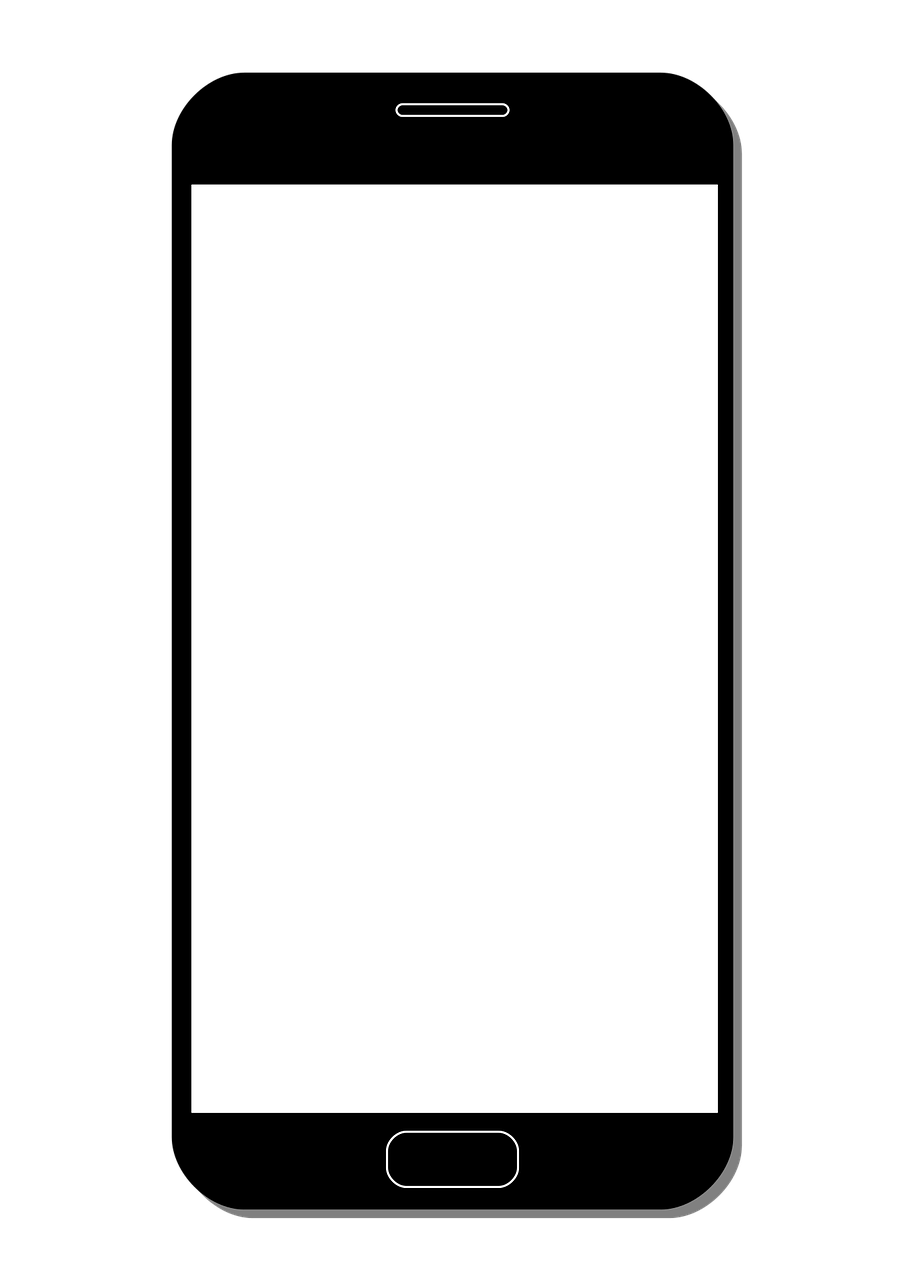
\includegraphics[width=1cm]{phone.png} 
& 
\includegraphics[width=1cm]{adventurer.png} 
& 
\includegraphics[width=2cm]{kangourou.png} \\

\includegraphics[width=1.5cm]{researcher.png} & $\leftarrow$
& 
\includegraphics[width = 1.5cm]{cloud.png}
& & &   \\
& & & 
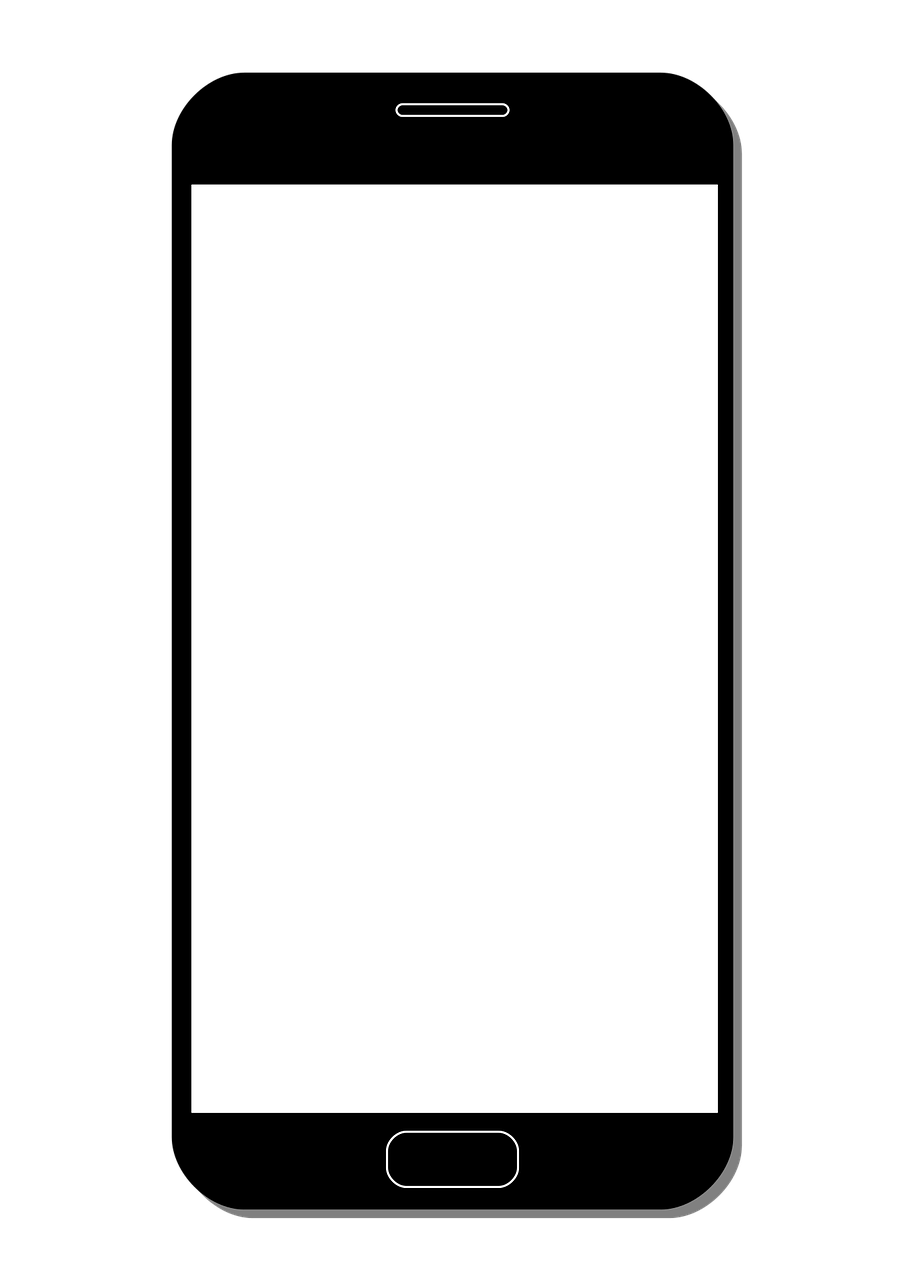
\includegraphics[width=1cm]{phone.png} 
& 
\includegraphics[width=1cm]{adventurer.png} 
& 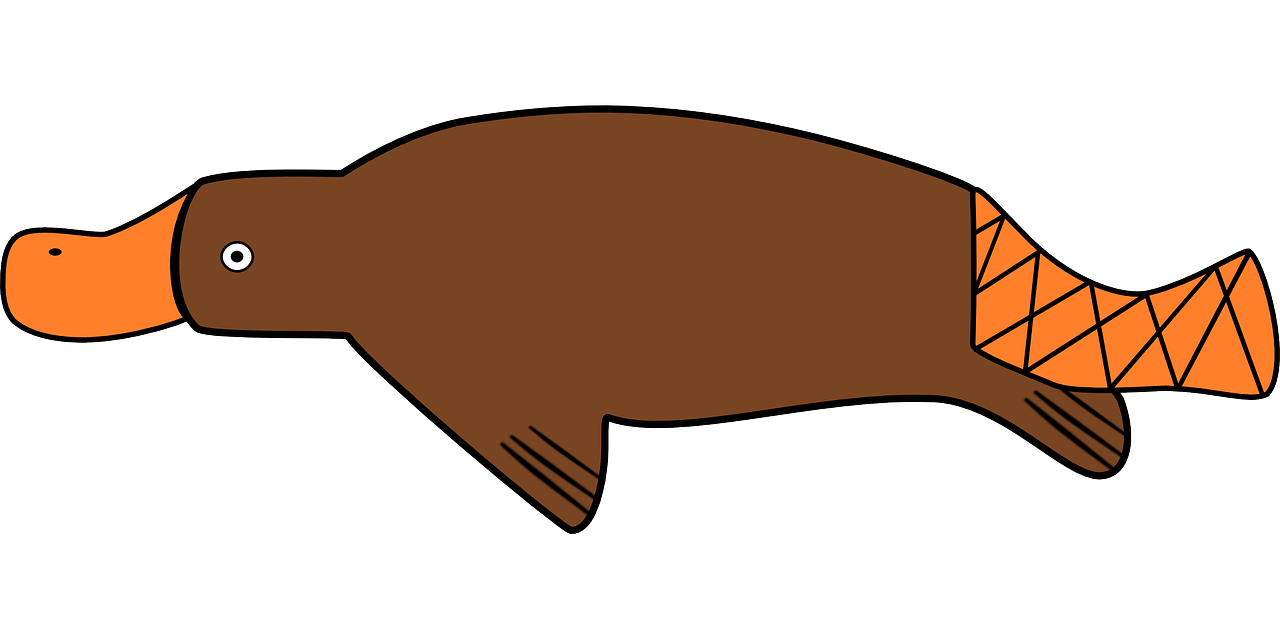
\includegraphics[width=2.5cm]{orni.png}
\end{tabular}
\end{frame}

\begin{frame}{Exemple fil rouge}
Exemple de données collectées:
\begin{itemize}
\item Animal vu (kangourou, ornithorynque)
\item Date
\item Lieu
\item Nom de l'aventurier
\item $\dots$
\end{itemize}
\end{frame}

\section{Concepts manipulés et travail antérieur}

\subsection{Confidentialité}
\begin{frame}{Confidentialité}
Un problème de confidentialité est défini par
\begin{itemize}
\item Qu'est-ce qu'on veut protéger?
\item De qui veut-on le protéger?
\end{itemize}
\end{frame}

\begin{frame}{Contraintes de confidentialité}
Dans l'exemple on veut protéger 
\begin{itemize}
\item L'association (date, lieu)
\item Les noms des aventuriers
\end{itemize}
\end{frame}

\begin{frame}{Hypothèses sur l'attaquant}
\begin{alertblock}{On ne fait confiance}
\begin{itemize}
\item Ni aux nuages utilisés
\item Ni au réseau utilisé
\end{itemize}
\end{alertblock}

\begin{exampleblock}{On fait confiance}
\begin{itemize}
\item A la machine de l'utilisateur.
\end{itemize}
\end{exampleblock}

\end{frame}

\subsection{Techniques de protection}
\begin{frame}{Chiffrement}
\begin{center}
\begin{block}{Définition}
Transformer l'information intelligible en inintelligible
de façon réversible pour les destinataires. 
\end{block}

\begin{exampleblock}{Exemple}<2>
\begin{center}
$\leftrightarrow$ \hspace*{1cm}
\end{center}
\begin{tabular}{lcr}
\begin{tabular}{ccc}
		Ana  & Melton	    & 4/8 \\
		Fred & Tamworth 	& 5/8 \\
		Ana  & Orange 		& 6/8
\end{tabular} & &
\begin{tabular}{ccc}
		LD6h736B  & Melton	    & 4/8 \\
		3ghjKrE	  & Tamworth 	& 5/8 \\
		LD6h736B  & Orange 		& 6/8
\end{tabular} \\
%9 juillet à 14h09	& & LD6h736B3ghjKrE	\\
\end{tabular}
\end{exampleblock}
\end{center}
\end{frame}

\begin{frame}{Fragmentation verticale}
\begin{block}{Définition}
Séparer (géographiquement, par exemple)
deux informations pour rendre inintelligible leur association.
\end{block}

\begin{exampleblock}{Exemple}<2>
\begin{tabular}{lcr}
&	\begin{tabular}{ccc}
		Ana  & Melton	    & 9 août \\
		Fred & Dubbo	 	& 10 août \\
		Ana  & Orange 		& 11 août
	\end{tabular}
& \\
\begin{tabular}{c}
Melton \\
Dubbo \\
Orange
\end{tabular}
& &
\begin{tabular}{cc}
Ana 	& 9 août \\
Fred 	& 10 août \\
Ana 	& 11 août
\end{tabular}
\end{tabular}
\end{exampleblock}
\end{frame}

\begin{frame}{Calculs côté utilisateur}
\begin{center}
\begin{tabular}{c}
On fait confiance à la machine de l'utilisateur \\
$\Downarrow$ \\
Les informations traitées et stockées \emph{localement} \\
sont supposées en sécurité
\end{tabular}
\end{center}
\end{frame}

\subsection{Le langage C2QL et l'algèbre relationnelle}
\begin{frame}{Enjeux d'une application utilisant le nuage}
\begin{itemize}
\item Utilisation du nuage
\begin{itemize}
\item Disponibilité
\item Passage à l'échelle automatisable
\end{itemize}
\item Protection de la confidentialité
\item Performances
\end{itemize}
\end{frame}

\begin{frame}{Enjeux et protection de la confidentialité}
\begin{center}
\hspace{0.7cm}

\includegraphics[width=0.9\textwidth]{snps.png}
\end{center}
\end{frame}

\begin{frame}{Relations}
\begin{center}
\begin{tabular}{cccc}
		Nom	 & Lieu			& Date	  & Animal 			\\ \hline
		Ana  & Melton	    & 9 août  & Kangourou 		\\
		Fred & Tamworth 	& 10 août & Ornithorynque 	\\
		Ana  & Orange 		& 11 août & Ornithorynque	\\
\end{tabular}
\end{center}
\end{frame}

\begin{frame}{Ensemble des fonctions \uncover<3->{étendu}}
\begin{itemize}
\item Projection, $\proj$ \uncover<2->{, $\proj_{Animal}$}
\item Sélection,  $\sel$ \uncover<2->{, $\sel_{|Aujourd'hui - date| < 8 jours}$}
\item Jonction,   $\Join$ \uncover<2->{, $Observations \Join Aventuriers$}
\item Agrégation et réduction, $\group$ et $\operatorname{fold}$ \\
\uncover<2->{$\fold{Animal}{[nbK, esp \mapsto\mathrm{ if }(esp == Kang) (nbK+1)
\ \mathrm{ else }\ nbK]}{0} \circ \group_{date}$}
\item<3-> Fragmentation et défragmentation, $\frag$ et $\defrag$ \\
\uncover<4>{$\defrag \circ \frag_{Lieu}$}
\item<3-> Chiffrement et déchiffrement, $\crypt$ et $\decrypt$ \\
\uncover<4>{$\decryptArgs{AES}{Nom}\cryptArgs{AES}{Nom}$}
\end{itemize}
\end{frame}

\begin{frame}{Le langage C2QL}
\begin{block}{En algèbre relationnelle}
$\# KangF = \operatorname{countK} \circ \proj_{date, Animal} \circ \sel_{Nom = Fred \wedge |Aujourd'hui-date|<8}$
\end{block}

\begin{block}{En C2QL}
\begin{align*}
\# KangF = \defrag \circ  (\proj_\emptyset, & \operatorname{countK} \circ \proj_{date, Animal} \circ \\
& 
\sel_{\operatorname{AES}(Nom) = 3ghjKrE \wedge |Aujourd'hui-date|<8}) \\
& \circ \frag_{\{Lieu\}}  \circ \cryptArgs{AES}{Nom}  
\end{align*}
\end{block}
\end{frame}


\subsection{Les lois de commutation}
\begin{frame}{Développer un programme C2QL}
\only{\begin{block}{D'abord, écrire version locale}
$\operatorname{countK} \circ \proj_{date, Animal} \circ \sel_{Nom = Fred \wedge |Aujourd'hui-date|<8}$
\end{block}}<-2>

\only{\begin{block}{Ensuite, composer les protections/déprotection à droite}
\begin{align*}
\operatorname{countK} &\circ \proj_{date, Animal} \circ \sel_{Nom = Fred \wedge |Aujourd'hui-date|<8} \\
&\circ \defrag \circ \frag_{Lieu} \circ \decryptArgs{AES}{Nom} \circ \cryptArgs{AES}{Nom}
\end{align*}
\end{block}}<2->

\only{\begin{block}{Finalement, faire commuter les opérateurs}
\begin{align*}
\# KangF = \defrag \circ  (\proj_\emptyset, & \operatorname{countK} \circ \proj_{date, Animal} \circ \\
& 
\sel_{\operatorname{AES}(Nom) = 3ghjKrE \wedge |Aujourd'hui-date|<8}) \\
& \circ \frag_{\{Lieu\}}  \circ \cryptArgs{AES}{Nom}  
\end{align*}
\end{block}}<4>
\end{frame}


\section{Contribution}
\subsection{Définir formellement les fonctions de C2QL}

\begin{frame}{Choix à faire: Tuples ou fonctions?}
\begin{center}
\begin{tabular}{cccc}
		Nom	 & Lieu			& Date	  & Animal 			\\ \hline
		Ana  & Melton	    & 9 août  & Kangourou 		\\
		Fred & Tamworth 	& 10 août & Ornithorynque 	\\
		Ana  & Orange 		& 11 août & Ornithorynque	\\
\end{tabular}

\begin{align*}
f : & Nom \mapsto Fred , Lieu \mapsto Tamworth, \\& Date \mapsto 10/08, 
Animal \mapsto Ornithorynque 
\end{align*}
\end{center}
\end{frame}

\begin{frame}{Choix à faire: Expressivité ou restrictivité?}
\begin{center}
\begin{tabular}{c}
L'implémentation faite en Idris \\
évite déjà les erreurs de programmation \\
$\Downarrow$ \\
Pour les démonstrations, les définitions peuvent être expressives
\end{tabular}
\end{center}
\begin{exampleblock}<2>{Exemple}
	$$
	\begin{array}{llcl}
	\projDelta:	& r		& \mapsto		& 
					\{{l|}_{(\delta\cap \s(r)) \cup \{id\}} / l \in r \}
	\end{array}
	$$
\end{exampleblock}
\end{frame}



\subsection{Prouver la correction des lois}
\begin{frame}{Structure des preuves}
$$
\left\lbrace
\begin{array}{cc}
res_1 = & (f \circ g) (r) \\
res_2 = & (g \circ f) (r)
\end{array}
\right.
$$
\begin{itemize}
\item Égalité des schémas relationnels
\item Inclusion de $res_1$ dans $res_2$
\item Inclusion de $res_2$ dans $res_1$
\end{itemize}
\end{frame}

\begin{frame}{Erreurs corrigées: projection et projection}
\begin{block}{Loi 3 page 30 de la thèse}
$$ 
\proj_{a_1} \circ \dots \circ \proj_{a_n} 
\equiv \proj_{a_1, \dots, a_n}
$$
\end{block}
\begin{block}{Contre-exemple}
\begin{tabular}{lr}
		a\(_{\text{1}}\) & a\(_{\text{2}}\)\\
		\hline
		a & 1\\
		b & 2\\
\end{tabular}

\(\pi_{a_1} \circ \pi_{a_2} (r) = \emptyset\)
mais
\(\pi_{a_1, a_2} (r) = (r)\)
\end{block}
\begin{exampleblock}{Correction}
$$
\proj_{\delta_1} \circ \dots \circ \proj_{\delta_n} 
\equiv \proj_{\delta_1 \cap \dots \cap \delta_n}
$$
\end{exampleblock}
\end{frame}

\begin{frame}{Erreurs corrigées : Defragmentation et projection}
\begin{block}{Loi 12 page 64 de la thèse}
$$
\projDelta \circ \defrag
\equiv \defrag \circ (\proj_{\delta \cap \delta'} , \proj_{\delta \setminus \delta'})
$$
\end{block}
\begin{exampleblock}{Correction}
\begin{align*}
\projDelta \circ \defrag
& = \defrag \circ (\proj_{\delta \cap \delta_1}, \proj_{\delta \cap \delta_2})
& \text{si $\delta_1 \cap \delta_2 = \emptyset$}
\end{align*}
\end{exampleblock}
\end{frame}

\subsection{Compléter l'ensemble de lois}

\begin{frame}{Critère de complétude}
Toutes les paires de fonctions possibles soient considérées
\end{frame}

\begin{frame}{Tableau des lois}
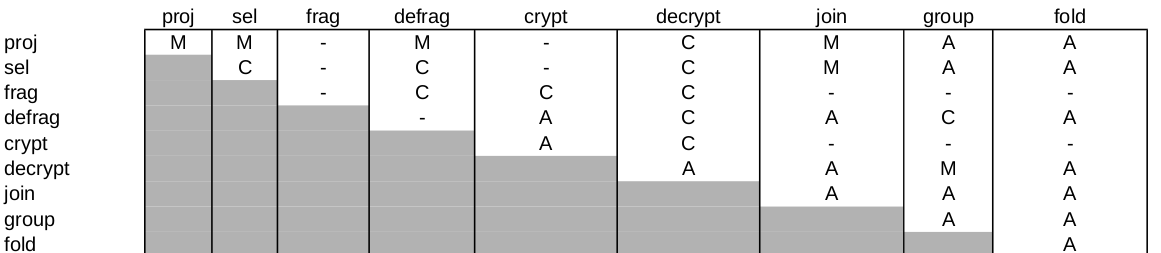
\includegraphics[width=\textwidth]{complLoisBilan.png}
\end{frame}

\begin{frame}{Exemple}
Soit $\delta_1$ le schéma relationnel du premier
	argument et $\delta_2$ le schéma relationnel du deuxième
	argument.
En appelant $(P)$ la propriété
\og Soit $\ch$ est injectif, soit $\alpha \notin \delta_1 \cap \delta_2$\fg{},
\begin{align}
\decryptCAlpha \circ \Join
& \equiv
\Join \circ (\decryptCAlpha, \id)
& \text{si $\alpha \in \delta_1$ et $(P)$} \\
\decryptCAlpha \circ \Join
& \equiv
\Join \circ (\id, \decryptCAlpha)
& \text{si $\alpha \in \delta_2$ et $(P)$} 
\end{align}
\end{frame}

\subsection{Une première version de l'optimiseur}
\begin{frame}{Automatiser l'optimisation}

\includegraphics[width = 0.5\textwidth]{work.png}
\end{frame}

\section{Travail futur}

\begin{frame}

\begin{block}{Autres pistes à explorer}
\begin{itemize}
\item Autres propriétés de sécurité
\item Autres mécanismes
\item Compilateur C2QL $\rightarrow$ application concrète
\item Finir compilateur vers Provérif
\item $\dots$
\end{itemize}
\end{block}

\end{frame}

\section*{Conclusion}
\begin{frame}{Conclusion}
\end{frame}

\end{document}